% pour genree un pdf: faire
% pdflatex exemple.tex
\documentclass{report}
\makeatletter
\def\@makechapterhead#1{
\vspace*{50\p@}
  {\parindent \z@ \raggedright \normalfont
    \ifnum \c@secnumdepth >\m@ne
      \if@mainmatter
        %\huge\bfseries \@chapapp\space \thechapter
        \Huge\bfseries \thechapter.\space%
        %\par\nobreak
        %\vskip 20\p@
      \fi
    \fi
    \interlinepenalty\@M
    \Huge \bfseries #1\par\nobreak
    \vskip 40\p@
  }}
\makeatother
%% Paquets LateX utiles

\usepackage[utf8]{inputenc} 		% encodage des caracteres utilise (pour les caracteres accentues) -- non utilise ici.
%\usepackage[latin1]{inputenc} 		% autre encodage
\usepackage[french]{babel}		% pour une mise en forme "francaise"
\usepackage[T1]{fontenc} 
\usepackage{amsmath,amssymb,amsthm}	% pour les maths
\usepackage{graphicx}			% pour inclure des graphiques
\usepackage{float}
\usepackage[hidelinks]{hyperref}
\usepackage{color}			% pour ajouter des couleurs dans vos textes
\usepackage{geometry}
\usepackage{tabularx}
\usepackage{caption}
\setlength\abovecaptionskip{0pt}
\geometry{hmargin=2.5cm,vmargin=3cm}
\renewcommand{\contentsname}{\centering Contents}




\begin{document}
\begin{titlepage}
    \begin{flushleft}
    
\includegraphics[width=11em]{images/logo.png}\\[1.5cm]
    \end{flushleft}
    \begin{center}
        \textsc{{\LARGE \color{blue} Master Données, Apprentissage et Connaissances-DAC}}\\[5cm]
        \textsc{\huge{RAPPORT PROJET DAC}}\\[1cm]
        \textsc{\vspace{10pt}\Huge{Clustering pour les infrastructures sans fils}}\\[3cm]
        \begin{minipage}{1\textwidth}
            \begin{flushleft} \large
            \textsc{\LARGE{Realisé par :}}\\[0.5cm]
            \textsc{Hanane Djeddal}\\
            \textsc{Liticia Touzari}\\[1.5 cm]
            \textsc{\LARGE{Encadré par :}}\\[0.5cm]
            \textsc{Anastasios Giovanidis}\\
            \end{flushleft}
        \end{minipage}
        \vfill
    \end{center}
  \end{titlepage}

 
  \vspace*{\stretch{0.5}}
  \begin{center}
    \section*{\LARGE{Résumé}}
\end{center}
    \paragraph{}
  \Large{
    L'augmentation croissante du trafic de données a posé de grands défis aux opérateurs mobiles pour augmenter leur capacité de traitement des données,
    ce qui entraîne une consommation d'énergie et des coûts de déploiement importants sans avoir necéssairement une croissance
    dans le chiffre d'affairs vu que l'utilisateur attend qu'il paye moins pour plus de données. Avec l'emergence de l'architecture Cloud Radio Access Network (C-RAN) 
    les unités de traitement des données peuvent désormais être centralisées et partagées entre les stations de base, chose qui 
    réduit les coûts de déploiement et offre une architecture de base qui facilite l'implémentation des algorithmes et des solutions pour des
    problèmes divers. Le partage des unités de traitement se fait en clusterisant les stations de base et en mappant 
    chauqe cluster à une unité de traitement de données. Les schémas de trafic des stations de base étants très dynamiques à différents moments et endroits,
    par exemple le trafic dans une région résidentielle durant la journée n'est pas le même durant la nuit, L'idée est de créer des
    cluster de stations de base avec des schéma de trafic complémentaires afin que l'unité de traitement peut être pleinement 
    utilisée à différentes périodes de temps, et la capacité requise à déployer devrait être inférieure à la somme des capacités d'une seule base stations. 
    Cependant, il est difficile de prévoir et de caractériser les schémas de trafic à l'avance pour réaliser des schémas de regroupement optimaux.
    Dans ce rapport, nous abordons ces problèmes en étudiant les solutions déjà proposées dans le cadre d'optimisation C-RAN basé sur l'apprentissage en profondeur.
    Premièrement, nous implémentons les algorithmes déjà existants, nous procédons par la suite à évaluer leur performances en utilisant des dataset fournit par Orange. 
    Nous exposons aussi des différents alogorithmes de clustering, principalement K-means, et nous essayons à les adapter à notre problème. 
    Nous terminons par comparer les performances des différentes méthodes. \\[2cm]
  \textbf{Mots clés: }
  C-RAN, RAN Cloudification, Clustering, K-means  
  }
  \vspace*{\stretch{1}}
  

  \tableofcontents
   


\newpage
\chapter{État de l'art}
\paragraph{}
  Dans cette partie, on va introduire les technologies et concepts principaux dans le projet. D'un part, on parle de l'architecture traditionnelle
  des réseaux sans fils et son évolution à l'architecure C-RAN. D'autre part, on présente deux méthodes de clustering: 
  K-means et le clustering héirarchique dans leur version la plus générale. À la fin, on introduit la methode de clustering proposée dans l'artcile [3]
  qu'on va implémenter et evaluer dans la suite du rapport. 
\section{L'architecture D-RAN}
\paragraph{}
Dans l'architecture traditionnelle Distributed Radio Access Network (D-RAN), le site de chaque cellule (eNodeB) contient deux compsants:
une unité de traitement de bande de base (BBU) au pied de la tour et une tête radio à distance (Remote Radio Head, RRH) au sommet. 
Les deux conposants sont reliés par un cable en fibre optique. Le RRH s’occupe des fonctionalités radio telles que conversion des 
fréquences, amplifications, A/D et D/A conversion etc. Quant à la BBU, elle effectue les traitements de la bande de base, des packets, etc et assure le fonctionnement de la station. 
\begin{figure}[h]
  \centering
  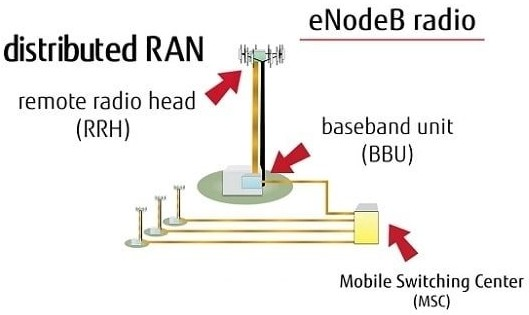
\includegraphics[width=25em]{images/D-RAN.jpg} 
  \caption{D-RAN}
\end{figure}
\paragraph{}
Une solution pour accomomder le nouveau volume du trafic est de deployer plus de cellules de petite taille et reutiliser les fréquences. Cependant, cette approche 
necessite des coûts imporants d'installation et crée un problème d'interférence entre les cellules. \\
Un autre problème que engendre cette architecture est la consomation d'energie. En effet, les stations de base consomme le plus d'energie dans les réseaux sans fils et augmenter
le nombre de cellules c'est augmenter les coûts d'exploitation et l'emission du gaz carbonique, qui, bien évidemment, a un effet négative sur l'environement.\\
Une nouvelle architecture doit être capable d'offrir une solution à ces problèmes tout en garadant un revenue positif.
\section{L'architecture C-RAN}
\paragraph{}
L'architecture Cloud Radio Access Network (C-RAN) est un concept qui combine des technique de Centralisation, Collaboration et de
Virtulaisation pour offrir une performance aémlioré avec moins de coûts et moins de consomation d'energie (Clean RAN).
\paragraph{}
L'idée de C-RAN est de centraliser les différentes ressources de traitement de bande de base (les BBUs) pour créer un 'pool' qui gère dynamiquement 
l'allocation de ressources. Les composants de base dans une architecture C-RAN sont :
\begin{enumerate}
  \item BBU pool : regroupe l’ensemble BBUs dans un centre et permet l’allocation dynamique et le reconfiguration basée sur des données en temps-réel.
  \item RRH : Comme dans les architectures traditionnelle, les RRHs sont distribués dans les différentes station de base et assurent les mêmes fonctionalités de couverage des signaux.
  \item Réseau de transmission : une interconnexion entre une instance de BBU et un RRH.
\end{enumerate}
\begin{figure}[h]
  \centering
  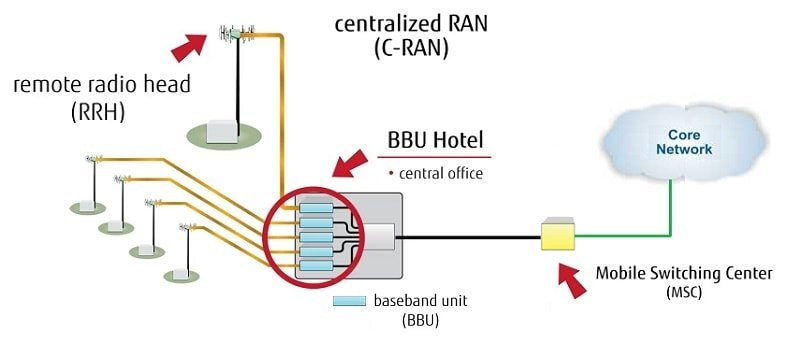
\includegraphics[width=25em]{images/C-RAN.jpg} 
  \caption{C-RAN}
\end{figure} 
\paragraph{}
Ce concept, simple et direct, offre plusieurs avantages. La centralisation des BBUs dans un seul pool avec des interconnexions 
qui relient les différents noeuds avec une bande passante elevée et une faible latance, permet la communication et l'echange d'information et par 
conséquence plusieurs technologies telles que Joint Processing et cooperative multiPoint (CoMP), difficile à implémenter dans l'architecture traditionnelle, seront facitement intégrées. 
En plus, contrairement à l'architecture traditionnelle où les ressources d'une BBU sont limitées à la station de base où elle est installée, dans le contexte C-RAN, 
les ressources sont aggrégées dans un pool (ressources cloudification) et peuvent être allouées sur demande, ce qui réduit la consomation d'energie et optimise l'utilisation des ressources. 
Aussi, due à sa nature basée sur le concept de Cloud et centralisation, C-RAN est caractérisée par sa flexibilité et scalabilité qui sont necessaires pour l'évolution des systèmes 5G.  

\section{Méthodes de Clustering}
\paragraph{}
Le clustering fait référence à un ensemble très large de techniques pour rechercher des sous-groupes, ou clusters, dans un ensemble de données. Lorsque nous regroupons les observations d'un ensemble de données, nous cherchons à les diviser en groupes distincts afin que les observations au sein de chaque groupe soient assez similaires les unes aux autres, tandis que les observations dans différents groupes sont assez différentes les unes des autres. Bien sûr, pour concrétiser cela, nous devons définir ce que signifie que deux ou plusieurs observations soient similaires ou différentes. En effet, il s'agit souvent d'une considération spécifique au domaine qui doit être faite sur la base de la connaissance des données étudiées.
Le clustering étant populaire dans de nombreux domaines, il existe un grand nombre de méthodes de clustering. Nous nous concentrons sur les deux approches de clustering les plus connues: le clustering K-means et le clustering hiérarchique. Dans le clustering K-means, nous cherchons à partitionner les observations en un nombre prédéfini de clusters. En revanche, dans le clustering hiérarchique, le nombre de clusters n'est pas prédéfini, nous nous retrouvons avec une représentation visuelle arborescente des observations, appelée dendrogramme, qui permet de visualiser immédiatement les regroupements obtenus pour chaque nombre possible de regroupements, de 1 à n. 
En général, nous pouvons regrouper des observations sur la base des caractéristiques afin d'identifier des sous-groupes parmi les observations, ou nous pouvons regrouper des caractéristiques sur la base des observations afin de découvrir des sous-groupes parmi les caractéristiques. [3]
\subsection{K-means Clustering} 
\paragraph{}
Le clustering K-means est une approche simple et élégante pour partitionner un ensemble de données en K clusters distincts qui ne se chevauchent pas. Pour effectuer le clustering K-means, nous devons d'abord spécifier le nombre souhaité de clusters K; alors l'algorithme K-means assignera chaque observation à exactement l'un des K clusters. 
La figure ci-dessous montre les résultats obtenus en déroulant l'algorithme sur l'ensemble des RRHs de Lille (ville Française) avec 88 emplacement différents.

\begin{figure}[h]
  \centering
  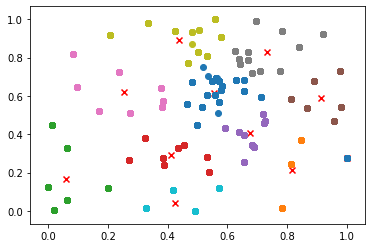
\includegraphics[width=25em]{images/k-means_lille.png}
  \caption{K-means clustering}
\end{figure}

La procédure de clustering K-means résulte d'un problème mathématique simple et intuitif. Nous commençons par définir une notation. Soit C1,. . . , CK désignent des ensembles contenant les indices des observations dans chaque cluster. Ces ensembles satisfont deux propriétés:
\begin{enumerate}
\item $C_{1} \cup C_{2} \cup ... \cup C_{k}=\lbrace1,...,n\rbrace$ chaque observation appartient à au moins l'un des K clusters.
\item $C_{k} \cap C_{k'}= \varnothing $ aucune observation n'appartient à plus d'un cluster.
\end{enumerate}
Par exemple, si la ième observation se trouve dans le kième groupe, alors $i \in C_{k}$. L'idée derrière le clustering K-means est qu'un bon clustering est celui pour lequel la variation intra-cluster est aussi petite que possible. La variation intra-cluster pour le cluster $C_{k}$ est une mesure $W(C_{k})$ de la différence entre les observations au sein d'un cluster. Par conséquent, nous voulons résoudre le problème :
$\min_{C_{1}, C_{2}, ... C_{K}}\sum^K_{k=1}C_{k}$. [3]

En termes, cette formule dit que nous voulons partitionner les observations en K clusters de telle sorte que la variation totale intra-cluster, additionnée sur tous les K clusters, soit aussi petite que possible.\\
Il s'agit en fait d'un problème très difficile à résoudre avec précision, car il existe presque $K^{n} $ façons de partitionner n observations en K clusters. Néanmoins, il existe un algorithme très simple pour fournir un optimum local - une assez bonne solution - au problème d'optimisation K-means. Cette approche est présentée dans le pseudo l'algorithme suivant :\\
\rule{\linewidth}{.1pt} 
\Large{Algorithme} K-means Clustering\\
\rule{\linewidth}{.1pt} 
\begin{enumerate}
\item Attribuez au hasard un numéro, de 1 à K, à chacune des observations.
Celles-ci servent d'initialisations.
\item Itérez jusqu'à ce que les affectations de cluster cessent de changer: 
\begin{enumerate}
\item Pour chacun des K clusters, calculer le centroïde du cluster.
\item Attribuez chaque observation au cluster dont le centroïde est le plus proche (où le plus proche est défini en utilisant la distance euclidienne par exemple).
\end{enumerate}
\end{enumerate}
\rule{\linewidth}{.1pt} 

Parce que l'algorithme K-means trouve une optimisation locale plutôt que globale, les résultats obtenus dépendront de l'affectation initiale (aléatoire) de chaque observation à l'étape 1 de l'algorithme. Pour cette raison, il est important d'exécuter l'algorithme plusieurs fois à partir de différentes configurations initiales aléatoires. Ensuite, en sélectionner la meilleure solution, c'est-à-dire celle pour laquelle l'objectif est le plus petit.\\
Comme vu précédemment, pour effectuer un clustering K-means, il faut définir le nombre de clusters K dés le départ. Le problème de la sélection de K est loin d'être simple. 

\subsection{Clustering Hierarchique}
\paragraph{}
Un inconvénient potentiel de l'algorithme K-means est qu'il faut pré-spécifier le nombre de clusters K. Le clustering hiérarchique est une approche alternative qui ne nécessite pas un choix particulier de K. Le résultat du clustering est souvant traduit par une représentation arborescente attrayante des observations, appelée dendrogramme.\\

Le dendrogramme du clustering hiérarchique est obtenu via un algorithme extrêmement simple. Commençant par définir une sorte de mesure de dissimilarité entre chaque paire d'observations. Le plus souvent, la distance euclidienne est utilisée. L'algorithme se déroule de manière itérative. Partant du bas du dendrogramme, chacune des n observations est traitée comme son propre cluster. Les deux clusters qui se ressemblent le plus sont ensuite fusionnées pour qu'il y ait  n - 1 clusters. Ensuite, les deux clusters qui se ressemblent le plus sont fusionnés à nouveau, de sorte qu'il en reste  n - 2 clusters. L'algorithme procède de cette manière jusqu'à ce que toutes les observations appartiennent à un seul cluster et que le dendrogramme soit terminé.\\
L'algorithme de clustering hiérarchique est donné comme suit:\\
\rule{\linewidth}{.1pt} 
\Large{Algorithme} Clustering Hiérarchique\\
\rule{\linewidth}{.1pt} 
\begin{enumerate}
\item Commencez par n observations et une mesure (telle que la distance) et traitez chacun observation comme un cluster.
\item Pour i= n, n-1, ..., 2: 
\begin{enumerate}
\item Examinez toutes les dissemblances inter-cluster par paires parmi les i clusters et identifiez la paire de clusters qui sont les moins dissemblables (c'est-à-dire les plus similaires). Fusionnez ces deux clusters. La dissimilarité entre ces deux groupes indique la hauteur dans le dendrogramme à laquelle la fusion doit être placée.
\item Calculez les nouvelles dissemblances inter-cluster par paire parmi les i-1 clusters restants.
\end{enumerate}
\end{enumerate}
\rule{\linewidth}{.1pt}
Le concept de dissimilarité entre une paire d'observations doit être étendu à une paire de groupes d'observations. Cette extension est obtenue en développant la notion de lien, qui définit la dissimilarité entre deux groupes d'observations. Les quatre types de liens les plus courants - complet, moyen, unique et centroïde - sont brièvement décrits dans le tableau ci-dessous:\\[0.5cm]
\begin{tabularx}{\linewidth}{|x|X|}
   \hline
  Linkage & Description  \\
  \hline
  Complet & Différenciation intercluster maximale. Calculez toutes les disparités par paires entre les observations du cluster A et les observations du cluster B, et retenir la plus grande de ces différences. \\
  \hline
  Unique & Dissimilarité intercluster minimale. Calculez toutes les disparités par paire entre les observations du cluster A et les observations du cluster B et noter la plus petite de ces différences. Un couplage unique peut entraîner des clusters étendues dans lesquelles des observations uniques sont fusionnées une par une. \\
  \hline
  Moyen & Dissimilarité intercluster moyenne. Calculez toutes les disparités par paires entre les observations du cluster A et les observations du cluster B et notez la moyenne de ces différences. \\
  \hline
  Centroïde & La dissimilarité entre le centroïde du cluster A et le centroïde du cluster B. La liaison centroïde peut entraîner des inversions indésirables. \\
  \hline
\end{tabularx}

\section{L'algorithme DCCA}
\paragraph{}
Pour optimiser l'utilisation des ressources, et maximiser l'utilié des unités de traitement de base, l'association BBU-RRH doit prendre 
en considération les variation du trafic. En effet, la demande de trafic de données n'est pas uniformément distribuée sur les différentes régions et période du temps (voir figure 4).
Donc, c'est important de regrouper des RRHs avec des schémas de trafic complémentaire afin que l'unité de traitement peut être pleinement 
utilisée à différentes périodes de temps. L'algorithme Distance-Constrained Complementarity-Aware (DCCA) est une méthode proposée par [3]
qui permet de trouver des schéma de clustering optimaux pour maximiser l'utilité de la capacité et réduire les coûts.

\begin{figure}[h]
  \centering
  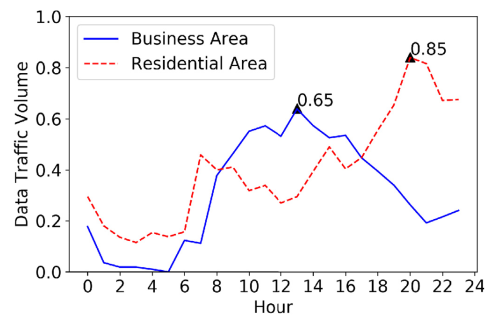
\includegraphics[width=25em]{images/trafic.png}
  \caption{Volume de trafic}
\end{figure} \\

L'algorithme introduit une mesure de complémentarité entre les RRHs utilisée pour calculer la connéctivité entre un RRH et un cluster.
L'objectif de DCCA est d'avoir une connectivité entre un RRH 'r' et son cluster qui est supérieure à la connectivité entre'r' et tout autre cluster.\\
$\forall v\in C_{k}$  Con(v,C) $\ge$ max $Con(v,C_{l}),C_{l} \in P$ \\
Dans la méthode proposée, une étape de prédiction de trafic précède l'application de DCCA. Pour chaque RRH, un pattern de trafic 
est prédit pour une duré de temps future basé sur l'historique du trafic du RRH. Un model Multivariate Long Short-Term Memory (MuLSTM) est utilisé 
pour générer une matrice F. L'algorithme MuLSTM prend un $F_{i}$ et retourne un $F_{i+1}$ tel que Fi est une matrice de dimension [Nt,Nr] avec, Nt: nombre de time slots et Nr: nombre des RRHs.\\
Ce modèle est utilisé pour prédire le trafic heure par heure pour le jour suivant. Le clustering des RRHs sera mit à jour dynamiquement selon ce trafic prédit. \\
L'étape suivante est l'application de DCCA. Avant d'introduire l'algorithme, on va définir quelque mesures.\\
\subsection{Définitions}
\begin{enumerate}
  \item \textbf{Distribution de peak hours :} Pour un cluster donné C, on recupère peak hours des RRHs du cluster, soit T. 
  On calcule par la suite l'entropie de shannon sur les probabilité d'avoir un peak-hour dans le cluster. 
  Une grande valeur de l'entropie implique une grande uncertitude ce qui veut dire une grande dispersion entre 
  les peak hours dans le cluster.\\
  H(C) = - $\sum_{k=1}^{K}p_{k} \log p_{k}$ \\
  Où K=|T(C)| et $p_{k}$ est la propabilité d'observer le peak hour correspondant dans l'ensemble T(C).
  \item \textbf{L'utilité de la capacité :} Le trafic aggréger des RRHs du cluster doit être proche à la capacité de la BBU du cluster sans la dépasser.\\
  $U(C)= \left(\frac{meanf(C)}{|B|}\right)^{\ln\frac{meanF(C)}{|B|} }$ 
  \item \textbf{Complémentarité :} $M(C) = U(C)*H(C)$
  \item \textbf{Matrice de complémentarité :} Il faut prendre en considération la distance entre les RRHs pour que les délais 
  de propagation entre BBU et RRH respectent les contraintes de qualité de service, et aussi pour permettre la communication 
  entre RRHs. Donc on définit un $\tau$ tel que les RRHs qui sont séparés par une distance > $\tau$ ne sont pas regroupés ensemble. 
  La matrice de complémentarité a la forme [Nr,Nr] et associe à chaque couple(ri,rj) la valeur :
  $w(ri,rj)= M({ri,rj})*a_ij$ tel que $a_ij = \begin{cases}
    1 & \text{si $dist(r_i,r_j) < \tau$,} \\
    0 & \text{sinon.}
    \end{cases}$ 
  \item \textbf{Connectivité :} Elle représente la mesure de distance qui permet d'affecter un RRH à un cluster:      $con(v,C)=\sum_{v'\in C}w_{vv'}$ \\
  Il faut prendre en considération de plus la distance entre le RRH et les autres clusters, on definit donc : \\
  $value(v,C)=con(v,C)*\log{\left(\frac{\tau}{max{dist(v,v')}}\right)} $ 
  \item \textbf{Clusters adjacents :} $\mathbb{C}(v)= {C| con(C,v) >0, C \in \mathbb{P}} $
\end{enumerate}

\paragraph{}
L'algorithme DCCA peut être, donc, décrit comme suit :\\
\rule{\linewidth}{.1pt} 
\Large{Algorithme} DCCA\\
\rule{\linewidth}{.1pt} 
\begin{enumerate}
\item Attribuez au hasard un numéro, de 1 à K, à chaque RRH.
Ils servent comme clusters initiaux.
\item Itérez jusqu'à ce que les affectations de cluster cessent de changer, ou on atteint le nombre max d'itérations: 
\begin{enumerate}
\item Pour chaque RRH, on calcule les clusters adjacents : AC.
\item Parmi les clusters de AC, on recupère celui qui a le value(v,C) max, soit newC).
\item Si newC est different de l'ancient cluster de RRH, on reaffecte RRH au nouveau cluster.
\end{enumerate}
\end{enumerate}
\rule{\linewidth}{.1pt} 

\chapter{Conception}

\section{Analyse des données}
\paragraph{}
Dans cette section on va analyser les données de géo-localisation et de trafic fournies par l'opérateur Orange pour les villes française: Paris, Nantes, Lille et Lyon.
\subsection{Données Géographiques}
\paragraph{}
Les données géographiques représentent les positions des RRHs sur un plan 2D (coordonnée x et y).\\
\subsubsection{Analyse des données pour la ville Lille}
\paragraph{}
- Nombre de RRHs est 1394 et le nombre de régions est de 88 RRHs (avec des RRHs à la même position).\\
\paragraph{}
- Cellules géographiques : le digramme de Voronoi ci-dessous permet de délimiter les zones géographiques dont est responsable chaque RRH et ainsi calculer la superficie de la zone :\\
\begin{figure}[H]
\begin{center}
  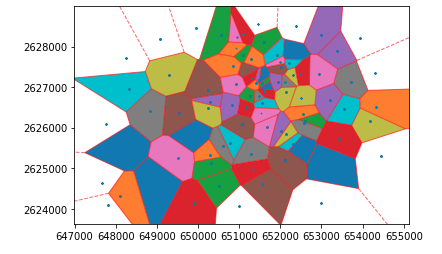
\includegraphics[scale=0.6]{images/voronoi-areas.png}\\
  \caption{Diagramme de Voronoi pour Lille}   
  \label{fig:picture}
\end{center}
\end{figure}
\paragraph{}
- Pour chaque RRH on évalue le nombre RRHs à distance variante de celui-ci:\\
Exemple : Pour le RRH à la position (649540, 2626350) on obtient les graphes suivants avec un pas de 500 m:\\
\begin{figure}[H]
  \centering
  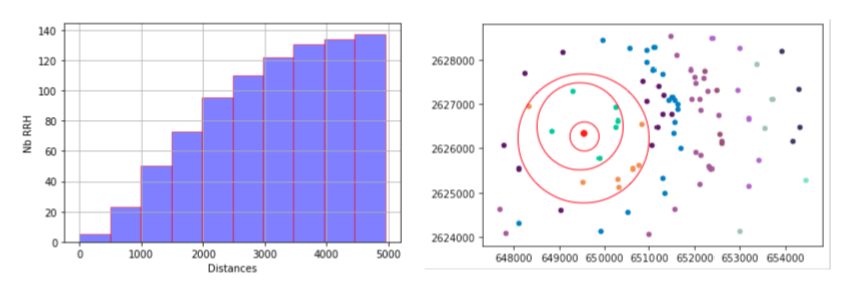
\includegraphics[scale=0.6]{images/histogramme_rrh_dist.png}
  \caption{Histogramme du nombre de RRHs par distance d'un point}   
  \label{fig:picture}
\end{figure}
\subsection{Données de Trafic}
\subsubsection{Analyse des données pour la ville Lille}
\paragraph{}
Les données de trafic renseignent pour chaque RRH le nombres de bytes up et bytes down pour des timeslot des 10min entre les mois de mars et juin 2019 ainsi que le maximum et minimum des bytes en up et down pour les RRHs.\\
Les courbes suivantes représentent le trafic up et down pour un RRH donné:\\

\begin{figure}[!htb]
   \begin{minipage}{0.48\textwidth}
     \centering
     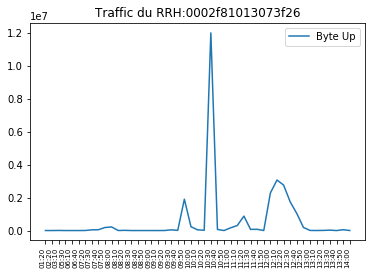
\includegraphics[scale=0.6]{images/byteUp1.png}
     \caption{Byte Up matin}\label{Fig:Data1}
   \end{minipage}\hfill
   \begin{minipage}{0.48\textwidth}
     \centering
     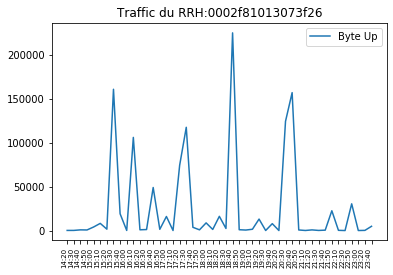
\includegraphics[scale=0.6]{images/byteUp2.png}
     \caption{Byte Up aprés 14h }\label{Fig:Data2}
   \end{minipage}
\end{figure} 
\begin{figure}[!htb]
   \begin{minipage}{0.48\textwidth}
     \centering
     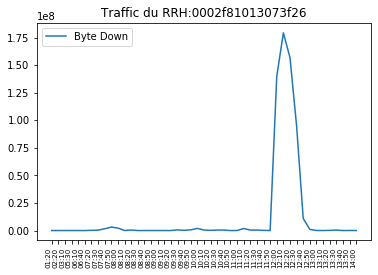
\includegraphics[scale=0.6]{images/byteDn1.png}
     \caption{Byte Down matin}\label{Fig:Data1}
   \end{minipage}\hfill
   \begin{minipage}{0.48\textwidth}
     \centering
     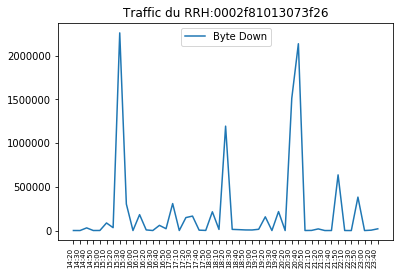
\includegraphics[scale=0.6]{images/byteDn2.png}
     \caption{Byte Down aprés 14h }\label{Fig:Data2}
   \end{minipage}
\end{figure} 
\begin{figure}[!htb]
   \begin{minipage}{0.48\textwidth}
     \centering
     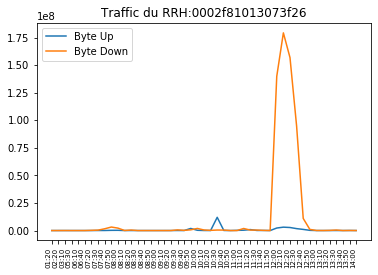
\includegraphics[scale=0.6]{images/byte1.png}
     \caption{Comparaison Byte Up et Byte Down matin}\label{Fig:Data1}
   \end{minipage}\hfill
   \begin{minipage}{0.48\textwidth}
     \centering
     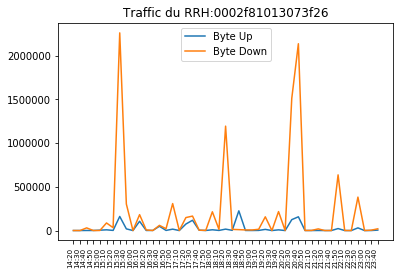
\includegraphics[scale=0.6]{images/byte2.png}
     \caption{Comparaison Byte Up et Byte Down aprés 14h }\label{Fig:Data2}
   \end{minipage}
\end{figure} 

On remarque bien que le trafic en down est beaucoup plus élevé qu'en up, et on peut facilement repérer les pics de trafic.\\
Les figures ci-dessous représente pour des périodes et jours différents le trafic RRH dans les régions du digramme de voronoi avec un code couleur.
\begin{figure}[!htb]
   \begin{minipage}{0.4\textwidth}
     \centering
     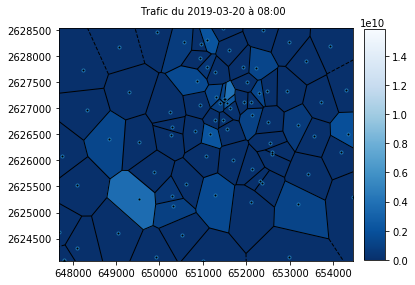
\includegraphics[scale=0.6]{images/8_20.png}
     \caption{Jour de semaine}\label{Fig:Data1}
   \end{minipage}\hfill
   \begin{minipage}{0.4\textwidth}
     \centering
     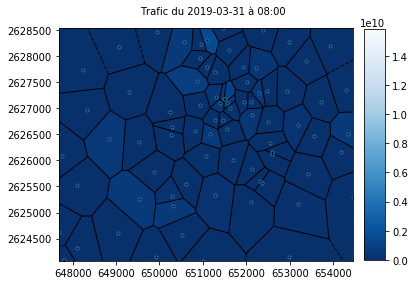
\includegraphics[scale=0.6]{images/8_31.png}
     \caption{Weekend}\label{Fig:Data2}
   \end{minipage}
\end{figure} 
\begin{figure}[!htb]
   \begin{minipage}{0.4\textwidth}
     \centering
     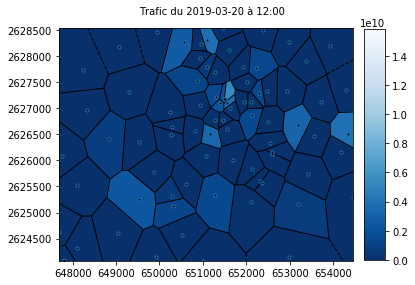
\includegraphics[scale=0.6]{images/12_20.png}
     \caption{Jour de semaine}\label{Fig:Data1}
   \end{minipage}\hfill
   \begin{minipage}{0.4\textwidth}
     \centering
     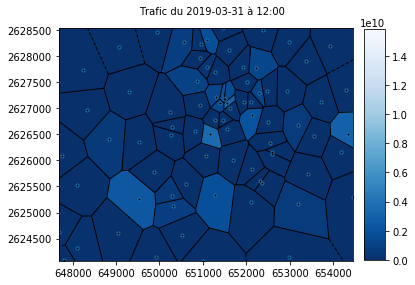
\includegraphics[scale=0.6]{images/12_31.png}
     \caption{Weekend }\label{Fig:Data2}
   \end{minipage}
\end{figure} 
\begin{figure}[!htb]
   \begin{minipage}{0.4\textwidth}
     \centering
     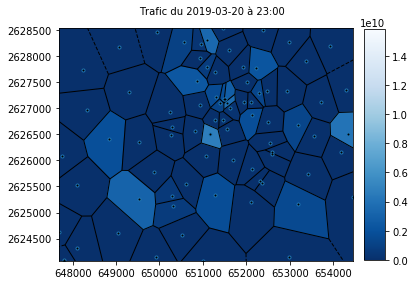
\includegraphics[scale=0.6]{images/23_20.png}
     \caption{Jour de semaine}\label{Fig:Data1}
   \end{minipage}\hfill
   \begin{minipage}{0.4\textwidth}
     \centering
     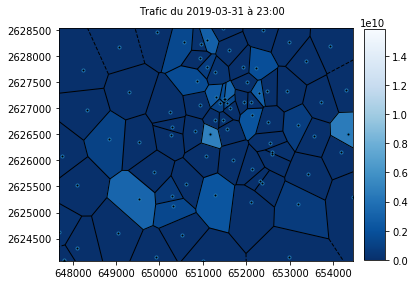
\includegraphics[scale=0.6]{images/23_31.png}
     \caption{Weekend }\label{Fig:Data2}
   \end{minipage}
\end{figure} 

\vspace*{\stretch{0.5}}

\end{document}